 %---------------------------------------------------------------------------------------
\documentclass[11pt]{article}
\usepackage[left=2.2cm, right=2.2cm, top=3cm, bottom = 3cm]{geometry}

\newenvironment{eg}[1]{
\begin{tcolorbox}[colback = white!15, arc=0pt,outer arc=0pt, colframe = black]
{\color{black} \textbf{Example.} #1} \\[5pt]
}
{
\end{tcolorbox}
}

\newdimen\diaw \diaw=1.5cm
\def\diamondscheme#1#2#3#4{%
    \vbox to\diaw{
       \kern-1ex
       \hbox to\diaw{\hss$#1$\hss}
       \vss
       \hbox to\diaw{\hbox to0pt{\hss$#2$\hss}\hss
                     \raise.7ex\hbox{\diacross}\hss
                     \hbox to0pt{\hss$#3$\hss}}
       \vss
       \hbox to\diaw{\hss$#4$\hss}
       \kern-1ex
    }
}
\newcount\tmpnum 
\tmpnum=\diaw 
\divide\tmpnum by65781  % tmpnum is now equal to \diaw in bp units
\divide\tmpnum by2
\def\tmp{\the\tmpnum\space}
\edef\diacross{\pdfliteral
   {q 0.4 w -\tmp \tmp m \tmp -\tmp l S -\tmp -\tmp m \tmp \tmp l S Q}}
\def\bigskip{\vskip\bigskipamount}

\usepackage{amsfonts,amsmath,amssymb,enumerate,mathtools, amsthm, soul, color, fancyhdr, hyperref, tcolorbox, algorithm}
\usepackage[noend]{algpseudocode}
\usepackage{polynom}
\usepackage{wrapfig}
\newcommand{\Mod}[1]{\ (\mathrm{mod}\ #1)}
\newcommand{\nl}{\\[5pt]}
\newcommand{\lstspacing}{\setlength\itemsep{1pt}}
\pagestyle{fancy}
\fancyhf{}
\rhead{Sajid Bashar - \thepage}
%\usepackage{tgpagella}
\lhead{MATH 239: NOTES}
\begin{document}
\makeatother
\parindent=0pt
\allowdisplaybreaks

\pdfinfo{
   /Author (Sajid Bashar)
   /Title  (MATH 239: Introduction to Combinatorics)
}

\begin{titlepage}
   \begin{center}
       \vspace*{7cm}
       {\huge \textbf{MATH 239: Introduction to Combinatorics}}
       \vspace{0.25cm}
              
       {\Large{Spring 2022}}
       \vspace{1cm}
       
       {\Large{Sajid Bashar}}
       \vspace{1cm}

       
   \end{center}
\end{titlepage}
%---------------------------------------------------------------------------------------
\begin{center}
    {\textbf{\Large{ENUMERATION}}}
\end{center}
\vspace{-20pt}
\section{Counting}
\subsection{Definitions and Techniques}
$\cup$ is OR, $\cap$ is AND. We can consider expressions $\overbrace{(A \cup B)}$ and $\overbrace{(A \cap B)}$ each as sets themselves.\nl
$|A \cap B| = |A| \times |B|$, $|A \cup B| = \{x : x \in A \text{ or } x \in B\} = |A| + |B| - |A \cap B|$ (account duplicates). \nl
For $\{1,\dots, n\} = [n]$, there are $n!$ permutations, $\binom{n}{k} = \frac{n!}{k!(n-k)!}$ $k$-sized subsets, and $2^n$ subsets. 
\begin{eg}{Binary Strings with Exactly $k$ 1s.}
For $n$ positions $s_1, \dots, s_n$, we can select $k$ positions to have 1s. We can then fill the leftover positions with 0s, which does not cost anything since we know for certain where to place them, giving us no choices but to fill the empty positions. So there are $\binom{n}{k}$ of these binary strings. 
\end{eg}
Some helpful binomial coefficient identities:
\begin{itemize}
  \setlength\itemsep{1pt}
    \item $\binom{n}{k} = \binom{n}{n-k}$ since choosing $k$ is equivalent to not choosing $k$. 
    \item $\binom{n}{0} = 1 = \binom{n}{n}$ 
    \item $\binom{n}{2} = \frac{n(n-1)}{2}$
    \item $n \leq \binom{n}{2}$ since $\binom{n}{2} \sim \Theta(n^2)$ 
    \item $ \binom{n}{k} = \binom{n-1}{k} + \binom{n-1}{k-1}$  
\end{itemize}
For a tuple $\lambda$ with length $k$, $\lambda = (p_1, \dots, p_k) \in \mathbb{N}^k$. \nl
For $n$ elements and $t$ types, there are $\binom{n+t-1}{t-1}$ ways to form $n$. \nl
We can create a counting story with a meaning that makes sense to us, and encode this combinatorially.\nl 
Sets $S_0, \dots, S_n$ partition $S$ if $S = S_0 \cup \dots \cup S_n$ and $S_0 \cap \dots \cap S_n = \emptyset$. So $|S| = \sum_{k = 0}^ n |S_k|$

\subsubsection{Cartesian Product}
 Pairing of all elements in $S$ and $T$ together into a 2-sized tuple. For all $a \in S$ and $b \in T$, we have $$\{(a,b) : a \in S \text{ and } b \in T\}$$
The cartesian product is not commutative! So the order of the sets matter s.t. $A \times B 
\neq B \times A$.

\subsubsection{$S^*$ (Infinite Unions)}
$$S^* = S^0 \cup S^1 \cup S^2 \cup \dots = \bigcup_{k\geq0} S^k$$
where $S^0 = \{\epsilon\}$ and $S^{k}$ is taking the cartesian product $k$ times s.t. $\lambda = (p_1, \dots, p_k) \in S^k$. 

\subsection{Combinatorial Proofs}

\subsubsection{Combinatorial Interpretation (Double Counting)}

The LHS and RHS are interpreted as counting some mutual set $S$. We simply just express what each side does with $S$. Since they both count $S$ in their respective ways, they must be equal. 
\begin{eg}{Give a combinatorial proof that $\binom{m+n}{r} = \sum_{k=0}^r \binom{m}{r-k}\binom{n}{k}$.}
$Proof.$ Let $A$ and $B$ be disjoint sets s.t. $|A| = m$, $|B| = n$. Then $\binom{m+n}{r}$ is number of $r$-element subsets of $(A \cup B)$. We can also create an $r$-element subset of $(A \cup B)$ in the following ways: 
\begin{itemize}
\lstspacing
    \item Choose $r$ elements from $A$ and 0 elements from $B$: We have $\binom{m}{r}\binom{n}{0}$ many subsets.
    \item \makebox[0pt][r]{OR\hspace{0.6cm}} 
Choose $r-1$ elements from $A$ and 1 elements from $B$: We have $\binom{m}{r-1}\binom{n}{1}$ many subsets.
    \item \makebox[0pt][r]{OR\hspace{0.6cm}} $\vdots$
    \item \makebox[0pt][r]{OR\hspace{0.6cm}} Choose 0 elements from $A$ and $r$ elements from $B$: We have $\binom{m}{0}\binom{n}{r}$ many subsets. 
\end{itemize}
Therefore $\binom{m+n}{r} = \sum_{k=0}^r \binom{m}{r-k}\binom{n}{k}$ since we have counted $A \cup B$ in two ways. \qed
\end{eg}

% \[\text{Review Links}\begin{cases} 
%     \hspace{5pt} \text{\href{https://www.youtube.com/watch?v=7mOYew7aJUA}{Combinatorial Proof (Full Lecture)}} \nl
%     \hspace{5pt} \text{\href{https://www.youtube.com/watch?v=z2xgVM4M5-s}{Math Reasoning: Combinatorial Identities and Proofs}}\nl 
%     \hspace{5pt} \text{\href{https://www.youtube.com/watch?v=C0g_hGyeO30}{Combinatorial Proofs}}
%     \end{cases}
% \]
\subsubsection{Bijections}
These are useful for giving proofs where the LHS and RHS count two different sets, $S$ and $S'$. \nl
For sets $A$ and $B$, we can say that the LHS and RHS of an expression are equal if we can map each element of $A$ to $B$ and vice-versa (mutual bijection). Formally, $A \leftrightharpoons B$ if $f: A \rightarrow B$ and $g: B \rightarrow A$. \nl
We need to show that it's well-defined: $\forall(a \in \mathcal{A}, b \in \mathcal{B})$, then $g(f(a)) = a$ and $f(g(b)) = b$.\nl
Binary strings and ternary strings are an ideal set to biject to since they make for good counting. \nl 
Tip: Removing an element that exists and adding it in if it doesn't exist or some variant is common. Also, use venn diagrams for sets to visualize them and try small examples ($n = 3$ or $n = 4$). \vspace{-2pt}
\begin{eg}{Give a combinatorial proof that $\binom{n}{k} = \binom{n-1}{k} + \binom{n-1}{k-1}$.}
Let $S = \{1, \dots, n\}$ and $S' = \{1, \dots, n-1\}$. Let $A$ contain all $k$-element subsets of $S$ and $B$ contain all $(k-1)$-element subsets or $k$-element subsets of $S'$. $|A| = \binom{n}{k}$ and $|B| = \binom{n-1}{k-1} + \binom{n-1}{k}$ by definition, so we prove the claim by showing that $A \rightleftharpoons B$. \nl 
Define $f: A \rightarrow B$ as, 
$$f(X) = \begin{cases}
X &\text{ if } n \not\in X\\
X \backslash \{n\} &\text{ if } n \in X
\end{cases}$$
Define $g: B \rightarrow A$ as, 
$$g(Y) = \begin{cases}
Y &\text{ if } |Y| = k\\
Y \cup \{n\} &\text{ if } |Y| = k - 1
\end{cases}$$
By the construction of these functions, $g(f(X)) = X$ for all $X \in A$ and $f(g(Y)) = Y$ for all $Y \in B$. Therefore $f$ is a bijection, so $A \leftrightharpoons B$ and thus $|A| = |B|$.

\end{eg}

% \begin{eg}{Give a combinatorial proof that $\binom{m+n}{n} = \sum_{k=0}^n \binom{m}{k}\binom{n}{n-k}$.}
% \vspace{-10pt}
% $$S = \{(A, B): A \subseteq \{1, \dots, m \}, B \subseteq \{m + 1, \dots, m + n\}, |A \cup B| = n\}$$
% \hspace*{-4mm}  
% \includegraphics[scale=0.373]{Midterm Example.png}
% \end{eg}


\newpage

\section{Generating Series (Generating Functions)}
\subsection{Formal Power Series}
\subsubsection{Basic Properties}

Represent sequence $\{a_n\}$ with $A(x) = \sum_{k \geq 0} a_kx^k$ s.t. $a_k$ are coefficients and $x^k$ are indeterminates. 
\nl
Two FPS are same iff they have same coefficients for same powers. \nl 
$[x^n]$ is the {\it{coefficient of}} operator. The extraction itself is by a conversion to a FPS. Some properties:
\begin{itemize}
    \setlength\itemsep{1pt}
    \item $[x^n](x^\ell F(x)) = [x^{n-\ell}]F(x)$ 
    \item $[x^n](aF(x) + bG(x)) = a[x^n]F(x) + b[x^n]G(x)$
    \item $[x^n](F(x)G(x)) = \sum_{\ell = 0}^n ([x^\ell] F(x))([x^{n-\ell}] G(x))$
\end{itemize}
 FPS are always invertible. The inverse $A^{-1}(x) = B(x)$ iff $A(x)B(x) = 1$ and exists iff $[x^0]A(x) \neq 0$.
\subsubsection{Coefficient Extraction}
\begin{eg}{$[x^{23}]\frac{1+x^2}{(1-2x^3)^7}$}
$$[x^{23}](1+x^2)\frac{1}{(1-2x^3)^7} = [x^{23}] \frac{1}{(1-2x^3)^7} + [x^{23}]x^2\frac{1}{(1-2x^3)^7} = [x^{23}] \frac{1}{(1-2x^3)^7} + [x^{21}]\frac{1}{(1-2x^3)^7}$$
By N.B.T., 
\begin{align*}
    [x^{23}]\sum_{n \geq 0} \binom{n + 6}{6} (2x^3)^n + [x^{21}]\sum_{n \geq 0} \binom{n + 6}{6} (2x^3)^n
\end{align*}
$3 \not| \: 23$, but $3 \: | \: 21$ so we can extract $[x^{21}]$ from the second sum, yielding $2^{7}\binom{13}{6}$. 
\end{eg}

For a more general case, we can write $[x^n]$ as a piecewise. 
\begin{eg}{$[x^n]\bigg(\frac{x^2}{1-x^3}\bigg)^{2022}$}
    $[x^n] x^{4044} \frac{1}{(1-x^3)^{2022}} = [x^n] \sum_{n \geq 0} \binom{n + 2021}{2021} x^{3n+4044} = \begin{cases} 
        \binom{k + 2021}{2021} &\text{if } n = 3k + 4044, k \in \mathbb{N}\\
        0 &\text{otherwise}
    \end{cases}$ 
\end{eg}
\begin{eg}{$[x^n]\frac{x^{k-1}}{(1-x)^k}$}
$$[x^{n-(k-1)}]\frac{1}{(1-x)^k} = \binom{(n-k+1)-k+1}{k-1} = \binom{n}{k-1}$$
\end{eg}
\subsection{Defining a Generating Series for $S$}
For an arbitrary set $S$, we use a weight function $w$ to map each element of $S$ to some meaning. The result is a generating series that ``generates" information about $S$. More precisely, $$\Phi_S(x) = \sum_{\sigma \in S}x^{w(\sigma) = \gamma}$$
The weight function of $A$ cannot have infinite weight $n$. Also, cannot have $w(\sigma) = 0$ for $A^*$.  \nl
The coefficient $[x^n]$ tells us the number of elements of $S$ that exactly have weight $w(\sigma) = n$. \nl
The generating series can be finite $S_n$ or infinite $S$. We can use these series to help model these:
\begin{itemize}
    \setlength\itemsep{1pt}
    \item $(1+x)^n = \sum_{k=0}^n \binom{n}{k}x^k$ \hfill Binomial Theorem
    \item $\frac{1}{(1-x)^k} = \sum_{n\geq0}\binom{n + k -1}{k -1} x^n$ \hfill Negative Binomial Theorem
    \item $\frac{1}{1-x}= \sum_{n \geq 0} x^n = 1 + x+ x^2 + \dots$ \hfill  Geometric Series
    \item $\frac{A}{1-R} = (AR^0) + (AR^1) + (AR^2) + \dots $\hfill Generalized Geometric Series
    \item $\frac{1-x^{n+1}}{1-x}= \sum_{k \geq 0} x^k - \sum_{k \geq n} x^k=  1 + x+ \dots + x^n$ \hfill (Finite Geometric Series)
    \item $(1+x)^{\alpha} = \sum_{n \geq 0} \binom{\alpha}{n} x^n$ \hfill Binomial Series
\end{itemize}
Tip: $\frac{1}{1+x} = \frac{1}{1-(-x)} = \sum_{n \geq 0} (-x)^n$\nl
Shifting $\sum_{n = 0}^m $: Left by $\alpha$ $\leadsto x^{n+\alpha}$, Right by $\alpha \leadsto x^{n - \alpha}$. Remember to apply this $n \pm \alpha$ everywhere!


\subsection{Sum, Product, and String Lemmas}
Sum Lemma gives us the generating series of the disjoint union of two sets $S$ and $T$, more precisely
$$\Phi_{S \cup T}(x) = \Phi_S(x) + \Phi_T(x)$$
Product Lemma gives us the generating series of the cartesian product of $S$ and $T$, more precisely 
$$\Phi_{S \times T}(x) = \sum_{a \in S}\sum_{b \in T}x^{w_S(a) + w_T(b)} = \sum_{a \in S}x^{w_S(a)} \cdot \sum_{b \in T}x^{w_T(b)} = \Phi_S(x)\Phi_T(x)$$
String Lemma only holds if there are no elements in $S$ with weight 0. That is, $$\Phi_{S^*}(x) = \frac{1}{1-\Phi_S(x)}$$

\subsection{Integer Compositions}
\subsubsection{Properties}
Composition of $n$ is an ordered sequence $\overbrace{(c_1, c_2, \dots, c_k)}$ of $k$ positive integers s.t. $c_1 + \dots + c_k = |C| = n$. \nl
We say $S$ contains these compositions $\sigma = (c_1, \dots, c_k)$ (usually with constraints) of all possible $n$, and use the Product Lemma (above for visualization) along with the weight function: $$w(\sigma) = \sigma \implies w((c_1, \dots, c_k)) = w_{c_1}(c_1) + \dots + w_{c_k}(c_k) = c_1 + \dots + c_k \implies w(C) = |C|$$
to find an explicit formula, which works because of the Product Lemma. Remember that 0 cannot be a weight! So say if a part is even, then $E = \{2, 4, \dots\}$. Then extracting $[x^n]$ will give us how many compositions exist for a specific $n$ since we're generating a number set. \nl 
We can consider any $S$ as $k$ blocks, $S_k$, s.t. blocks are generated independently, then package them together using $\cap$ and $\cup$, and then use the Product Lemma on all $k$ blocks for $\Phi_{S_k}(x)$.\nl 
% For instance, the first part has some constraint and the remaining $k-1$ parts have another constraint. That is, 
% $$S = \rule{5mm}{0.4pt} \: \cap \rule{5mm}{0.4pt} \: \cap \rule{5mm}{0.4pt} \: \cap \dots \cap \rule{5mm}{0.4pt}$$
To generate all possible $k$, we use the String Lemma on $\Phi_{S_k}(x)$ since we need to generate all sizes.\nl
We're essentially deconstructing each $k$-tuple (composition) and deducing how they were generated. 

\subsubsection{Algorithm for Finding Integer Compositions}
\begin{enumerate}[(1)]
    \lstspacing
    \item Determine respective generating series that satisfy constraints of each part. 
    \item Package all generating series found in (1) into one generating series for $k$ parts given by $\Phi_{S_k}(x)$. Consider any constraints on $k$ s.t. $k$ implicitly implies a different $k$. Can there be 0 parts? 
    \begin{eg}{Empty Compositions}
    ``The first part is odd" implies that the first part exists so $k \implies k + 1$. ``All parts are odd" does not imply that a part exists. ``There is an even number of parts" does not imply that a part exists. ``The last part is divisible by 3" implies that the last part exists.
    \end{eg}
    \item If unknown number of parts, use String Lemma to generate  all possible $k$. So $\Phi_S(x) = \sum_{k \geq 0} \Phi_{S_k}(x)$.
    \item If needed, extract $[x^n]\Phi_{S}(x)$ to find all possible integer compositions of $n$. 
\end{enumerate}
Tip: Of $k$ parts, if exactly 2 parts are even $\implies$ $k-2$ parts are odd. Instead, if at least 2 parts are even $\implies$ $k-2$ parts are $\mathbb{N}$. Same idea works if we swap which parts are even and odd. \nl
Tip: Congruence relation is given by $a \equiv b \pmod n  \implies a = bk + n$. 
% \begin{eg}{Find generating series of $n$ such that the first part is not divisible by 3 and
% the other parts are $\geq$ 2 so $[x^n]$ counts the number of such integer compositions of $n$.}
% For $k$ parts use the Sum and Product Lemmas, 
% $$S_k = (S_{(1 \text{ mod } 3)} \cup S_{(2 \text{ mod } 3)}) \cap (\mathbb{N}_{\geq 2})^{k-1} \implies \Phi_{S_k}(x) = \bigg( \frac{x}{1-x^3} + \frac{x^2}{1-x^3}\bigg)\bigg (\frac{x^2}{1-x}\bigg)^{k-1}$$
% Now to generate all possible $k$-sized compositions we use the String Lemma to obtain
% \begin{align*}
%     \Phi_S(x) &= \sum_{k \geq 0} \Phi_{S_k} \\
%               &= \sum_{k \geq 0} \bigg( \frac{x}{1-x^3} + \frac{x^2}{1-x^3}\bigg)\bigg (\frac{x^2}{1-x}\bigg)^{k-1}\\
%               &= \frac{x+x^2}{1-x^3}\cdot \sum_{k \geq 0} \bigg (\frac{x^2}{1-x}\bigg)^{k-1}\\
%               &= \frac{x+x^2}{1-x^3}\cdot \frac{\frac{1-x}{x^2}}{1-\frac{x^2}{1-x}} &\text{\bigg($A= \frac{1-x}{x^2}$, $R =\frac{x^2}{1-x}\bigg)$}\\
%     \Phi_S(x) &= \frac{x+x^2}{1-x^3}\cdot \frac{\left(1-x\right)\left(1-x\right)}{x^2\left(1-x-x^2\right)}
% \end{align*}
% \end{eg}

\newpage
\section{Binary Strings}
Blocks are maximal substrings of one digit, like $\underbrace{0000}\underbrace{111}$. 

\subsubsection{Concatenation}
Concatenation of two strings $A$ and $B$ is analogous to taking the cartesian product but removing commas. More formally, $\{ab : a \in A \text{ and } b \in B\}$, like FOIL. Careful, this isn't commutative so it may cause ambiguity!
\begin{eg}{$A = \{0, 01, 011\}$, $B = \{1, 11\}$}
\vspace{-20pt}
\begin{align*}
    AB &= \{01, 011, 011, 0111, 0111, 01111\} \implies \text{Ambiguous}\\
    BA &= \{10, 101, 1011, 110, 1101, 11011\} \implies \text{Unambiguous}
\end{align*}
\end{eg}
% We can generate all binary strings (unambiguously) via infinite unions s.t. $A^n$ are concatenation powers,
% $$\{0, 1\}^* = \{\epsilon, (0), (1), (00), (11), (01), (10), (000), (101), \dots\}$$ 
\subsection{Regular Expressions}
Each regular expression $R$ recursively produces a corresponding set $\mathcal{R}$ of binary strings (rational language). Regex consists of, 
\begin{itemize}
\lstspacing
    \item $\epsilon, 0, $ or 1
    \item $R_1 \smile R_2$ (Union) \hfill (Choose $R_1$ or $R_2$)
    \item $R_1R_2$ (Concatenation) \hfill ($R_1$ followed by $R_2$) 
    \item $R^*$ (Concatenation Powers) \hfill (Include $R$ arbitrary times) 
\end{itemize}
Informally, we can interpret regex as a process to build a specific string in $\mathcal{R}$. \nl 
Tip: Treat $(R_1 \smile R_2)^*$ as infinite iterations, in each iteration we arbitrarily choose which to concatenate. 

\begin{eg}{$\mathcal{S}$ contains all strings s.t. each block of 1's is followed by a block of 0's of length one or four. Write an unambiguous regular expression that produces $\mathcal{S}$. }
\vspace{-10pt}
$$0^*(11^*00^*)^*1^* \implies 0^*(11^*(0 \smile 0000))^*$$
\end{eg}

We can also define a recursive regex in terms of itself: $$S = \epsilon \smile S(0 \smile 1)$$
Can also write $\{\epsilon\} \cup S\{0, 1\}$. This produces all binary strings, and reads as ``A string produced by $S$ is the empty string or a string produced by $S$ followed by 0 or 1".

\subsection{Ambiguity}
% A regular expression is unambiguous if when we concatenate sets of strings and can distinctly identify each substring to its corresponding original set.\nl
Regular expression $R$ is unambiguous if every string is produced exactly once (uniquely formed) in $\mathcal{R}$. Otherwise, $R$ is ambiguous.

\subsubsection{Proving Ambiguity}
Give example of a specific string that is produced in more than one way.

\begin{eg}{Show that $S = (11)^*10 \smile (11)^*11 \smile 0)^*(\epsilon \smile 1)$ is ambiguous.}
We can produce the binary string $\alpha = 1111111111$ in two ways using the expression $((11)^* 10 \smile (11)^{*} 11 \smile 0) \epsilon$. Note that we choose to concatenate the empty string using the expression $(\epsilon \smile 1)$. The first way to produce $\alpha$ is by first choosing $\epsilon(11)$ from the nested expression $(11)^{*} 11$, and then concatenating $(111111)11$ also from $(11)^{*} 11$. That is, $$\underbrace{11}\underbrace{11111111}$$ 
The second way to produce $\alpha$ is by first choosing (11)11 from the nested expression $(11)^{*} 11$, and then concatenating $(1111)11$ also from $(11)^{*} 11$. That is, $$\underbrace{1111}\underbrace{111111}$$
\end{eg}

\subsubsection{Proving Unambiguity}
Show REs separated by $\smile$ are disjoint, then we can say that RE is $\therefore$ unambiguous. \nl
Show concatenated REs $\leftrightharpoons$ with Cartesian product of rational languages they produce $(Lem \: 3.9)$.
\begin{eg}{Show that $S = (001 \smile 01 \smile 1)^*0^*$ is unambiguous.}
Each string produced has the form $\alpha\beta$ where $\alpha = (001 \smile 01 \smile 1)^*$ and $\beta = 0^*$. Notice that 001, 01, and 1 are disjoint and thus $01 \smile 001 \smile 1$ is unambiguous. $\alpha$ does not produce 0, so $\beta$ is unambiguously all copies of $0$ at the end of the string. All strings formed by $\alpha$ are of the form
    $$\underbrace{11...1}_k \mu \underbrace{11...1}_{k_1} \mu \underbrace{11...1}_{k_2}...$$
    where $\mu = 0$ or $\mu = 00$, $k \geq 0$, and $k_i \geq 1$. Given $k$, $k_1, k_2, \dots$ there is exactly one way to produce the string above that form from $(001 \smile 01 \smile 1)^*$. All strings produced by $0^*$ have the form $000\dots$ where $0$ is repeated $k' \geq 0$ times and so there is exactly one way to produce the string from $0^*$. 
\end{eg}

\subsection{Block Decomposition}
We break down binary strings by decomposing them into blocks.
To help us make unambiguous expressions, we can alter a known unambiguous expression that produces all binary strings in blocks by treating it like a template and substituting for each of the parts depending on $\mathcal{S}$ $(Cor. )$:
$$0^* (11^*00^*)^*1^* \text{ or } 1^*(00^*11^*)^*0^*$$
Other unambiguous expression templates include: $(0 \smile 1)^*$, $0^*(10^*)^*, 1^*(01^*)^*$ \nl
Tip: If constraint, for first and last block give option of using $\epsilon$.

\subsection{Recursive Block Decomposition}

\subsubsection{The Forbidden Substring $\alpha$}
$Proof \: Sketch.$
Let $S$ be the set of all binary strings that do not contain $\alpha$ as a substring, and let $T$ be the set of strings that have exactly one occurrence of $\alpha$, at the very end (that is, as a suffix). A string in $S \cup T$ is either empty, or it ends with either a 0 or a 1. Translating this into a relation is given as
$$S \cup T = \{\epsilon\} \cup S\{0, 1\}$$
which corresponds to the generating series of \begin{align}
    \Phi_S(x) + \Phi_T(x) = 1 + \Phi_S(x)(2x) 
\end{align}
Notice that the string $\alpha$ (= 1011101 for e.g.) can overlap itself in a nontrivial way. That is, 
\begin{center}
    \begin{tabular}{cccccc|ccccccc}
         . & . & . & . & . & . & 1 & 0 & 1 & 1 & 1 & 0 & 1\\
         \hline
         1 & 0 & 1 & 1 & 1 & 0 & 1 & $\uparrow$ & $\uparrow$ & $\uparrow$ & $\uparrow$ & $\uparrow$ & $\uparrow$\\
         . & 1 & 0 & 1 & 1 & 1 & \underline{0} & \underline{1} & . & . & . & . & .\\
         . & . & 1 & 0 & 1 & 1 & 1 & 0 & 1 & $\uparrow$ & $\uparrow$ & $\uparrow$ & $\uparrow$  \\
         . & . & . & 1 & 0 & 1 & \underline{1} & \underline{1} & \underline{0} & \underline{1} & . & . & .  \\
         . & . & . & . & 1 & 0 & \underline{1} & \underline{1} & \underline{1} & \underline{0} & \underline{1} & . & .  \\
         . & . & . & . & . & 1 & \underline{0} & \underline{1} & \underline{1} & \underline{1} & \underline{0} & \underline{1} & . \\
    \end{tabular}
\end{center}
Looking at all the possible ways that $\alpha$ can overlap itself, we see that in this case \begin{align}S\{\alpha\} = T\{\epsilon, \beta_1, \dots, \beta_k\}\end{align} 
By definition $T\{\epsilon, \beta_1, \dots, \beta_k\} \subseteq S\{\alpha\}$. To verify $S\{\alpha\} \subseteq T\{\epsilon, \beta_1, \dots, \beta_k\}$, we have to consider if $S$ can end with a proper prefix of $\alpha$ (not all) s.t. when $S$ is concatenated with $\alpha$ we may get two $\alpha$s (overlapping). All the bits on the LHS of the table are the possible endings that strings in $S$ can have. If all bits on the RHS match up with $\alpha$ (i.e. we can make two copies of $\alpha$), then take the bits with arrows and concatenate them and add them to the list of $\beta$s so $T$ also produces two $\alpha$s.

\subsection{Parsing Regular Expressions into Generating Series}
For a length function $\ell$, always define $w(\sigma) = \ell(\sigma)$. So $[x^n]\Phi_{\mathcal{S}(x)}$ is the number of binary strings of rational language $\mathcal{S}$ (made by $S$) with length $n$.  Factoring $\Phi_\mathcal{S}(x)$ is helpful for parsing recursive regex. \nl 
If $R = f(x)$ and $S = g(x)$, the parsing rules are:
\begin{itemize}
    \lstspacing
    \item $\epsilon \leadsto x^0 = 1$
    \item 0, 1 $\leadsto x^1$
    \item $R \smile S \leadsto f(x) + g(x)$
    \item $RS \leadsto f(x)g(x)$
    \item $R^* \leadsto \frac{1}{1-f(x)}$
\end{itemize}
\begin{eg}{Find $\Phi_{\mathcal{S}}(x)$ of $S = 0^{*}(11^{*}(0\smile0000))^{*}$.}
\vspace{-10pt}
$$\Phi_{\mathcal{S}}(x) = \frac{1}{1-x} \cdot \frac{1}{1 - (x \cdot \frac{1}{1-x} \cdot (x + x^4))}$$
\end{eg}

\newpage

\section{Recurrence Relations}
We use linear recurrences $\{a_n\}$ to help us find coefficients of rational functions $\frac{P(x)}{Q(x)}$. These sequences satisfy $\{a_n\} = 0$. \nl
In particular, when written in terms of $a_n$, then $a_n \iff [x^n]A(x)$.\nl 
Remember that the recurrence should be in terms of just $a_n$ (including not being $-a_n$). When dealing with any computation, always re-index the recurrence so that it relies on previous terms and not terms ahead. 

\begin{eg}{}
\vspace{-25pt}
$$a_{n+2}= 2a_n+a_{n+1} \implies a_n = 2a_{n-2} + a_{n-1}$$
\end{eg}

\subsubsection{Factoring Polynomials of Degree 2}
Always factor out $(-1)$ from $-a_2x^2$. 
$$\diamondscheme{AC}{\frac{}{A}}{\frac{}{A}}{B}$$

\subsubsection{Factoring Polynomials of Degree 3}
Say $a_3x^3 \pm a_2x^2 \pm a_1x \pm a_0$, try finding a root $x = \alpha$, then use synthetic division. 
$$\polyhornerscheme[x=-1]{1-3x^2-2x^3}$$
\subsubsection{Partial Fractions}
\begin{enumerate}[(1)]
    \item Factor $Q(x)$. Assign a partial fraction for each exponent from 1 up. 
    \item Try substituting roots and solving for unknown constants. Otherwise, solve system of equations.
\end{enumerate}

\subsection{Rational Power Series to Explicit Coefficient Formula $[x^n]$}
\begin{enumerate}[(1)]
    \lstspacing
    \item Factor $Q(x)$. 
    \item Partial fraction decomposition to create linearly independent RPS.
    \item Simplify, remember to preserve $[x^n]$ throughout calculation.   
\end{enumerate}
\begin{eg}{Find an explicit formula of $A(x) = \frac{3-20x}{1-10x+25x^2}$.}
\vspace{-15pt}
\begin{align*}
    [x^n] \frac{-4}{5x-1} + \frac{-1}{(5x-1)^2} &=  [x^n] \bigg(4 \cdot \frac{1}{1-5x} - \frac{1}{(1-5x)^2} \bigg)\\
    &= 4[x^n] \sum_{n \geq 0} (5x)^n -1 [x^n] \sum_{n \geq 0} \binom{n+1}{1}(5x)^n\\
    &= 4 \cdot 5^n - 1\cdot (n+1) \cdot 5^n\\
    &= 5^n (4 - (n + 1)) = 5^n(3 - n)
\end{align*}
\end{eg}

\subsection{Rational Power Series to Linear Recurrences}
$P(x)$ is initial terms and $Q(x)$ is the equation for the recurrence relation. Using $Thm. \: 4.8$, we read the RHS and give the equation as a piecewise with the convention that $a_n = 0$ if $n < 0$. Parsing algorithm:
\begin{enumerate}[(1)]
\lstspacing
    \item Convert $Q(x)$ into a recurrence relation set to zero and match each power of all terms $x^k$ to $a_{n - k}$. 
    \item Correspond each power of $P(x)$ s.t. $\alpha x^k \rightarrow ``\alpha, \text{ if } n = k"$ in the piecewise ($A(x) = \alpha$). Then, ``$0, \text{if } n \geq ( deg(Q(x)))$" in piecewise. 
    \item Find initial conditions up to $a_{deg(Q(x)) - 1}$ by setting recurrence relation from (2) to each $\alpha$ and solving for each $a_k$. 
\end{enumerate}
\begin{eg}{$A(x) = \frac{1+x-4x^2}{1-3x^2+2x^3}$}
From Theorem 4.8, we can read from the RHS of $A(x)$ that for all $n \in \mathbb{N}$:
    \[a_n - 3a_{n-2} + 2a_{n-3} =  \begin{cases} 
        1 &\text{if } n = 0\\
        1 &\text{if } n = 1\\
        -4 &\text{if } n = 2\\
        0 &\text{if } n \geq 3
    \end{cases}
    \]
    with the convention that $a_n = 0$ if $n < 0$. We can determine the initial conditions as follows: 
    \begin{align*}
        [x^0] &: a_0 = 1   \\
        [x^1] &: a_1 = 1 \\
        [x^1] &: a_2 - 3a_0 = -4 \implies a_2 = -1 
    \end{align*}
    The recurrence $a_n - 3a_{n-2} + 2a_{n-3}$ holds for all $n \geq 3$.
\end{eg}

\subsection{Linear Recurrences to Rational Power Series}
\begin{enumerate}[(1)]
\lstspacing
    \item Use initial conditions with our convention to find $\alpha$, then form $P(x)$.
    \item Convert recurrence to $Q(x)$ of rational function by matching $a_{n - k}$ to $x^k$. 
    \item If explicit formula for ${a_n}$ needed, use 4.1.
\end{enumerate}
\begin{eg}{$a_n - 10a_{n-1}+25a_{n-2}=0$ for $n \geq 2$, $a_0 =3$, $a_1 = 10$. Find RPS of $a_n$. }
By Theorem 4.8, reading the recurrence yields $Q(x) = 1 - 10x + 25x^2$. With the convention that $a_n = 0$ if $n < 0$ we solve $P(x)$ as, 
\begin{align*}
    \underline{n = 0} &: a_0 = 3\\
    \underline{n = 1} &: a_1 - 10a_0 = 10 - 10(3) = -20
\end{align*}
So $P(x) = 3 -20x$, therefore $$A(x) = \frac{3-20x}{1-10x+25x^2}$$
\end{eg}

\subsection{Linear Recurrences to Formulas of $a_n$ as Functions of $n$ (Explicit $[x^n]$ Formula)}
The conversion of the recurrence to $Q(x)$ is identical. We also use $Thm. \: 4.14$ which implies that there are constants for sufficiently large $n$ s.t. $a_n$ is a general formula. Then we use given recurrence terms to solve for these constants. The algorithm is:
\begin{enumerate}[(1)]
\lstspacing
    \item Convert $Q(x)$ into a recurrence relation set to zero and match each power of all terms $x^k$ to $a_{n - k}$. 
    \item Factor $Q(x)$. 
    \item Use (2) to find a general formula $a_n$ with constants s.t. each constant factor is degree $n - 1$ less. 
    \begin{eg}{}
    \vspace{-25pt}
     $$Q(x) = (1-2x)^2(1+x) \implies a_n = (A+Bn)2^n + C(-1)^n$$
    \end{eg}
    \item Solve for the unknown constants using the initial recurrence terms by setting $a_n$ to each term and solving simultaneous equations. 
\end{enumerate} 

\subsection{Catalan Numbers}
$$C_n = \frac{1}{n+1}\binom{2n}{n}$$

\newpage
\begin{center}{\textbf{\Large{GRAPH THEORY}}}\end{center}
\vspace{-20pt}
\section{Properties of Graphs}
\subsection{Basic Characterizations}
$G = (V(G), E(G))$ s.t. $V$ is vertices and $E$ has edges (unordered pairs of vertices). \nl
If $u$ and $v$ are neighbours, they are adjacent ($v \in N_G(u)$) and $uv$ is incident to $u$ and $v$. \nl 
$deg(v)$ is the number of edges incident with $v$. If $deg(v) = 0$, then $v$ is an isolated vertex. 

\subsubsection{Matrix Multiplication}
Number of rows in $A$ must equal number of columns in $B$, and their sizes $n$ also need to be the same. $c_{ij}$ is the dot product of the $i^{th}$ row of $A$ and $j^{th}$ column of $B$ where the dot product is multiplying term-by-term and summing them up. 
 $$
     \begin{pmatrix}
         a_{11} & a_{12} & \cdots & a_{1n}\\
         \vdots & \vdots & \ddots & \vdots\\ 
         a_{m1} & a_{m2} & \cdots & a_{mn} 
     \end{pmatrix}
     \times
     \begin{pmatrix}
         b_{11} & b_{12} & \cdots & b_{1p}\\
         \vdots & \vdots & \ddots & \vdots\\ 
         b_{n1} & b_{n2} & \cdots & b_{np} 
     \end{pmatrix}
      =
     \begin{pmatrix}
         c_{11} & c_{12} & \cdots & c_{1p}\\
         \vdots & \vdots & \ddots & \vdots\\ 
         c_{m1} & c_{m2} & \cdots & c_{mp} 
     \end{pmatrix}$$
 $$c_{ij}= a_{i1} b_{1j} + a_{i2} b_{2j} +\cdots+ a_{in} + b_{nj} = \sum_{k=1}^n a_{ik}b_{kj}$$

\subsubsection{Adjacency Matrix}
\[a_{ij}=  \begin{cases} 
        1, \text{if } v_i \text{ is adjacent to } v_j\\
        0, \text{ otherwise}
    \end{cases}
    \]

\subsubsection{Incidence Matrix}
Rows are vertices $v_i$, columns are edges $e_j$.
    \[b_{ij}=  \begin{cases} 
        1, \text{if } e_j \text{ is incident to } v_i\\
        0, \text{ otherwise}
    \end{cases}
    \]
Each row sum corresponds to the degree of a vertex and each column sum is always 2 (edges are incident to two vertices or loops are incident to themselves). The sum of all row sums is twice the number of edges (i.e. number of columns). 

\subsubsection{Handshaking Lemma}
$$2e = \sum_{v \in V(G)}deg(v)$$

This property must hold for all components of $G$, even if we remove any number of edges. \nl It also implies there is an even number of vertices with odd degree $(Cor\: 4.3.2)$. 

\begin{eg}{A vertex has degree 1 or 5. Show that $n_1 = \frac{5}{4}n - \frac{1}{2}e$}
\vspace{-20pt}
\begin{align}
    \setcounter{equation}{0}
    2e &= n_1 + 5(n_5)\\
    n = n_1 + n_5 \implies n_5 &= n - n_1
\end{align}
$$2e = n_1 + 5(n - n_1) \implies 2e = n_1 + 5n - 5n_1 \implies 4n_1 = 5n - 2e \implies n_1 = \frac{5}{4}n - \frac{1}{2}e $$
\end{eg}

\subsubsection{Edge Deletion}
We can remove an edge s.t. $G - e$ or $E(G) \backslash \{e\}$. \nl 
The Handshaking Lemma should still hold after $G - e$. 

\subsection{Isomorphisms}
Two graphs are isomorphic if one can be obtained from the other by renaming vertices while the structural property is preserved. Formally, it's a bijection $f: V(G) \rightarrow V(G')$ where for $v \in V(G)$ we have a corresponding $f(v) \in V(G')$ (for multigraphs, we need to find a bijection for the edges as well). \nl
The isomorphism class is the collection of graphs that are isomorphic to $G$. Up to isomorphism ($\forall$ classes) depends on the number of configurations of $G$ where the adjacency structures are all different. 
\subsubsection{Proving Two Graphs are Isomorphic}
Directly state a mapping for each vertex $v \in G$ to $G'$ in a table. Note that $f(v)$ is symmetric. \nl 
Tip: Compare the degrees and neighbours to identify the mapping. 
\begin{center}
\begin{tabular}{c|c}
 $v$ & $f(v)$ \\
 \hline
 \vdots & \vdots 
\end{tabular}
\end{center}

\subsubsection{Proving Two Graphs are Not Isomorphic}
Identify a graph invariant (property of $G$ that doesn't change under an isomorphism). Helpful ones:
\begin{itemize}
\lstspacing
    \item Degree Sequence (Non-decreasing sequence $(d_1, \dots, d_n)$) 
    \item Planarity 
    \item Bipartiteness
    \item Number of Triangles (Copies of $K_3$ or 3-cycles)
    \item Number of Cycles with the Same Length
\end{itemize}

\subsection{Classes of Graphs}
\subsubsection{Complete Graphs - $K_n$}
Each pair of vertices is an edge. All vertices are degree $n-1$, so there is $\binom{n}{2}$ edges. \nl  A complete bipartite is denoted $K_{m, n}$ where $m$ and $n$ are the respective sizes of vertex classes. 
\begin{eg}{$K_4$.}
\vspace{-30pt}
\begin{center}
    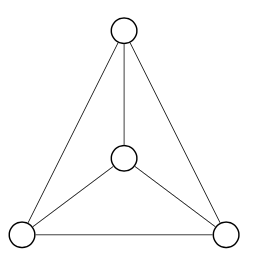
\includegraphics[scale=0.5]{Figures/K4.png}
\end{center}
\end{eg}

\subsubsection{$K$-Regular Graphs}
All vertices are degree $k$, so there are $\frac{nk}{2}$ edges.
\subsubsection{Bipartite Graphs}
A partition of vertices $(A,B)$ exists where each edge of $G$ joins one vertex in $A$ with $B$. \nl
$\sum_{v\in A}deg_G(v) = \sum_{v\in B}deg_G(v)$
\begin{eg}{$K_{2,3}.$}
\vspace{-30pt}
\begin{center}
    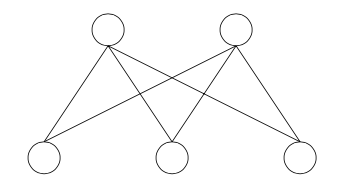
\includegraphics[scale=0.5]{Figures/Bipartite.png}
\end{center}
\end{eg}
Tip: Counting the number of edges for one vertex class gives us the number of edges for the other. 
\subsubsection{$n$-Cube (Hypercube)}
$V(G)$ is the set of all binary strings of length $n$. $N_G(v)$ consists of all binary strings that differ in exactly one position.\nl
Hypercubes are $n$-regular. All $n$ vertices have degree $n$, since from $n$ positions we choose $k = 1$ bits to flip which implies that a vertex has $\binom{n}{1} = n$ neighbours. So there's $n \cdot 2^{n-1}$ edges. \nl 
As an aside, this can be generalized further by noting that a Hamming distance of $k$ means choosing $k$ bits to be flipped, so that in general, any binary string of length $n$ has $\binom{n}{k}$ other strings at Hamming distance $k$.\nl
They are also bipartite, $A$ has all vertices with an odd number of 0s and $B$ with all vertices of an even number of 0s. 

\subsection{Walks and Paths}
The length is the number of edges. Trivial walks and paths have length 0. 

\subsubsection{$uv$-Walk}
Sequence of alternating vertices and edges $(u = v_0, v_0v_1, \dots, v_{k-1}v_k, v_k = k)$.

\subsubsection{$uv$-Path}
A $uv$-walk with no repeated vertices (thus no repeated edges). \nl 
If there is a $uv$-walk in $G$, there is a $uv$-path in $G$. The proof is by finding repeated vertices, removing the parts between the repetition, and repeating until no vertices repeat (use a shorter route). \nl 
If an $xu$-path and $uy$-path exist, then a $xy$-path exists $(Thm \: 4.6.2)$.

\subsection{Euler Tours (Euler Circuits)}
From a specific $v$, we visit every edge of $G$ exactly once and return to $v$ (closed walk). \nl
Euler Tours are only possible iff $\forall$ vertices are of even degree $(Thm \: 4.9.2)$. 

\subsection{Subgraphs and Cycles}

\subsubsection{Subgraphs}
$H$ is a subgraph if $V(H) \subseteq V(G)$, $E(H) \subseteq E(G)$. \nl 
If $V(H) = V(G)$, $H$ is a spanning subgraph. Also, if $H \neq G$ is a proper subgraph ($H$ is not $G$ itself). 

\subsubsection{Cycles}
A cycle is a subgraph with $k$ distinct vertices. They're $2$-regular graphs and are $uv$-paths + $uv$. \nl 
Cycles must at least have a length of 3 ($K_3$). 
If each vertex has at least degree 2, then $G$ contains a cycle. The proof is by the shortest path argument.\nl 
If there are two distinct paths from vertex $u$ to vertex $v$ in $G$, then $G$ contains a cycle $(Cor. \: 4.10.4)$. \nl
$Proof \: Sketch.$ Assume $P = v_0, \dots, v_k$ is the longest path. Since $v_0$ has degree at least 2, it has another neighbour $x$. If $x$ is not on the path, then $x, v_0, \dots, v_k$ is longer, contradiction. So $x = v_i$ for some $i \geq 2$, and $v_0, v_1, \dots, v_i, v_0$ is a cycle in $G$. \hfill \qedsymbol \nl

The girth is the length of the shortest cycle. If a cycle does not exist, the girth is infinity. \nl 
A spanning cycle is a Hamilton Cycle - we have to visit all the vertices exactly once.\nl
A graph is bipartite iff it has no odd cycles $(Thm \: 5.3.2)$.

\subsection{Connectedness}

\subsubsection{Components and Bridges}
Components are islands without bridges, or more formally maximally connected subgraphs of $G$. \nl
Bridges connect these islands together, where an edge $e$ is a bridge if $G-e$ gives more components of $G$ $(Thm \: 4.10.3)$ and is one iff it's not contained in any cycle of $G$. \nl
\begin{center}
    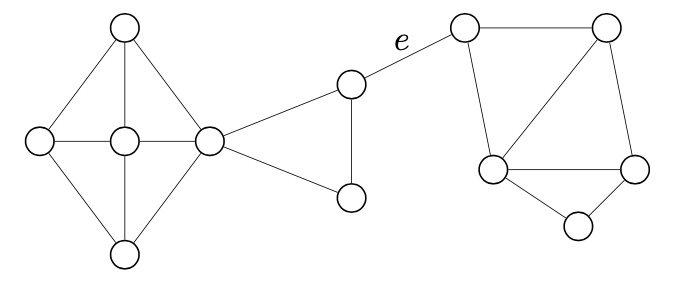
\includegraphics[scale=0.5]{Figures/Bridge.png}
\end{center}

The cut induced by $X \subseteq V(G)$ is the set of all edges in $G$ with precisely one end in $X$. It is essentially all the edges that are bridges between the vertices in whatever the cut is being induced as (i.e. $X$) with everything else it's connected to. It can be drawn as a line through the edges in the cut.


\subsubsection{Connected Graphs}
$G$ is connected if for all pairs of vertices $u$ and $v$, there is a path. So we can get from any point $A$ to $B$. \nl
If for each vertex $v$, there is a path from $v$ to $u$ then $G$ is connected. That is, if there's a path between a fixed vertex and each of the remaining vertices we say that $G$ is connected ($Thm \: 4.8.2$). \nl
If $V(H_1) \cap V(H_2) \neq \emptyset$, then $H_1 \cup H_2$ is connected s.t. $H_1 \cup H_2 = (V(H_1) \cup V(H_2), E(H_1) \cup E(H_2))$. 

\begin{eg}{Show that the $n$-cube is connected.}
The idea is that we can get to the vertex of $n$ 0's from an arbitrary vertex $v$. This can be done by continuously flipping the leftmost 1, since $N_{G_n}(v)$ is all binary strings that differ in 1 position. \nl
$Proof.$ Let $v_0 \in V(G)$ be the string of $n$ 0's. Let $x$ be any string of length $n$. Suppose $x$ has $k$ 1's at positions $i_1, \dots, i_k$. We produce $k$ strings as follows: $v_j$ is the string of length $n$ with exactly $j$ 1's, at positions $i_1, \dots i_j$. Then $v_j$ and $v_{j+1}$ differ in exactly one position $i_{j+1}$. So $v_jv_{j+1}$ is an edge. Then $v_0, v_1, v_2, \dots, v_k = x$ is a $v_0,x$-path. By Thm. 4.8.2, the $n$-cube is connected. \qed 
\end{eg}

%% CONSIDER INCLUDING HAMMING DISTANCE 

\subsubsection{Disconnected Graphs}
$G$ is not connected iff there exists a non-empty proper subset $X$ where the cut induced by $X$ is empty ($\emptyset$) $(Thm \: 4.8.5)$. So to show $G$ is disconnected, we need to show that the cut induced by $X$ is empty which means there's no edges between $X$ and $V(G) \backslash X$. \nl 
This implies that if $G$ is disconnected, there's at least two components.
\begin{center}
    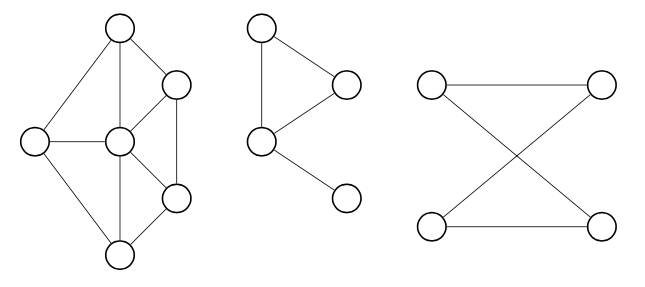
\includegraphics[scale=0.5]{Figures/Disconnected.png}
\end{center}
Tip: Imagine isolating each vertex in $X$ using a circle. 

\newpage 
\section{Trees}
\subsection{Properties}
(Minimally) connected graphs with no cycles.  
\begin{center}
    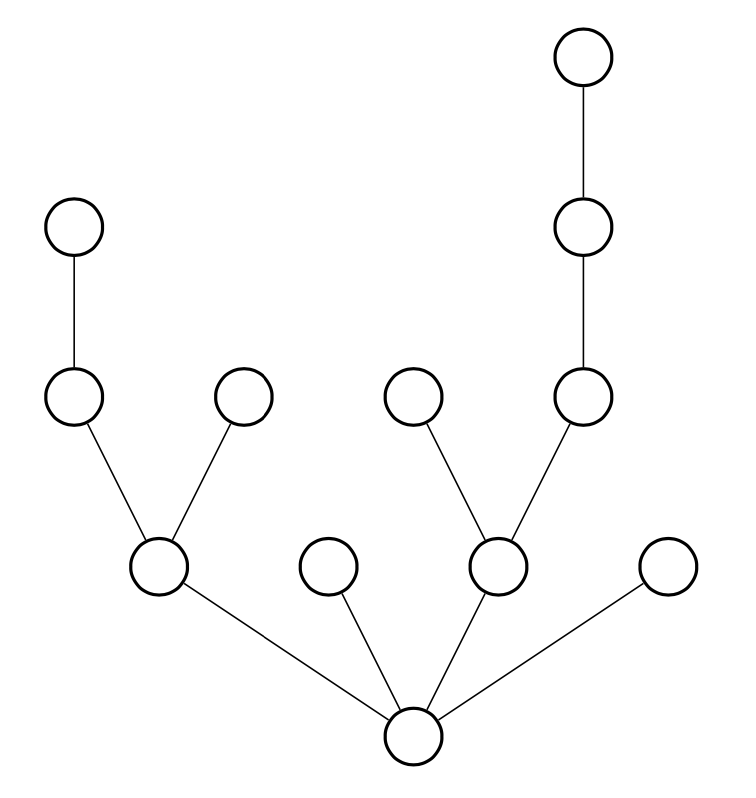
\includegraphics[scale=0.5]{Figures/Tree.png}
\end{center}
A forest is multiple trees. \nl
Every edge in $T$ is a bridge $(Lem. \: 5.14)$. The proof uses the fact that no edge is in a cycle. \nl
$\forall u, v \in V(T)$, there's a unique $u,v$ path in $T$ $(Lem. \: 5.1.3)$. \nl 
For trees, $m = n - 1$ (or $|E(G)| = |V(G)| - 1$) ($Thm. \: 5.15$). \nl 
If $G$ is connected and has $m = n- 1$ edges, then $G$ is a tree. \nl
More generally, for a forest with $k$ components, then $|E(G)| = |V(G)| - k$ $(Cor \: 5.16)$. \nl 
Leafs are vertices with degree 1. \nl 
Every $T$ with at least 2 vertices has at least 2 leaves $(Thm. \: 5.18)$. The proof is by the longest path argument. \nl 
Trees are bipartite. Bipartite graphs cannot contain odd cycles and trees don't have them anyways.
\subsection{Spanning Trees}
Spanning subgraphs that are trees. \nl 
A graph is connected iff it contains a spanning tree $(Thm \: 5.2.1)$. \nl
If $T$ is a spanning tree of $G$ and $e$ is an edge not in $T$, then $T+e$ contains exactly one cycle $C$. Moreover, if $e_0$ is any edge on $C$, then $T + e - e_0$ is also a spanning tree of $G$ ($Thm$ 5.2.3). \nl 
If $T$ is a spanning tree of $G$ and $e$ is an edge in $T$, then $T-e$ has 2 components. If $e_0$ is in the cut induced by one of the components, then $T - e + e_0$ is also a spanning tree of $G$ ($Thm$ 5.2.4). 

\newpage
\section{Planar Graphs}
\subsection{Properties of Planarity}
Graphs where all edges only intersect at their ends. The drawing is a planar embedding of $G$. 
\begin{center}
    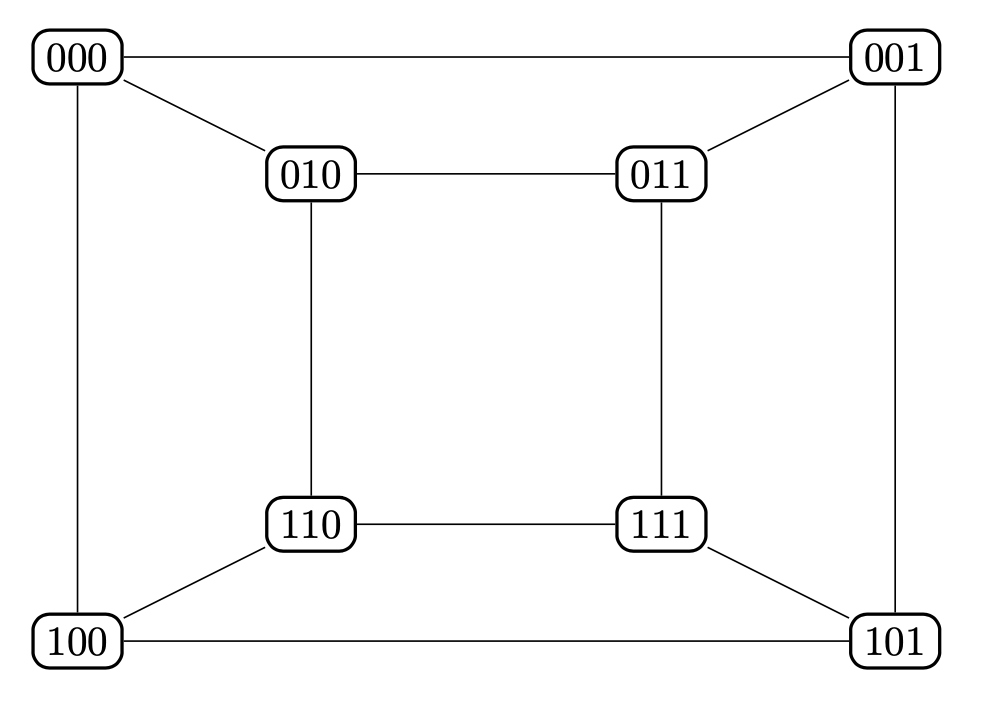
\includegraphics[scale=0.4]{Figures/Hypercube.png}
\end{center}
Planar embeddings partition the plane into faces (connected regions). The outer face is unbounded.
\subsubsection{Certifying Planar Graphs}
The only way to show that $G$ is a planar graph is to directly provide a planar embedding. 
\subsubsection{Faces}
The boundary of a face is all vertices and edges that touch the face. A boundary walk is a closed walk around the perimeter of the face walk. \nl
The degree of a face is the length of its boundary walk.  
\begin{center}
    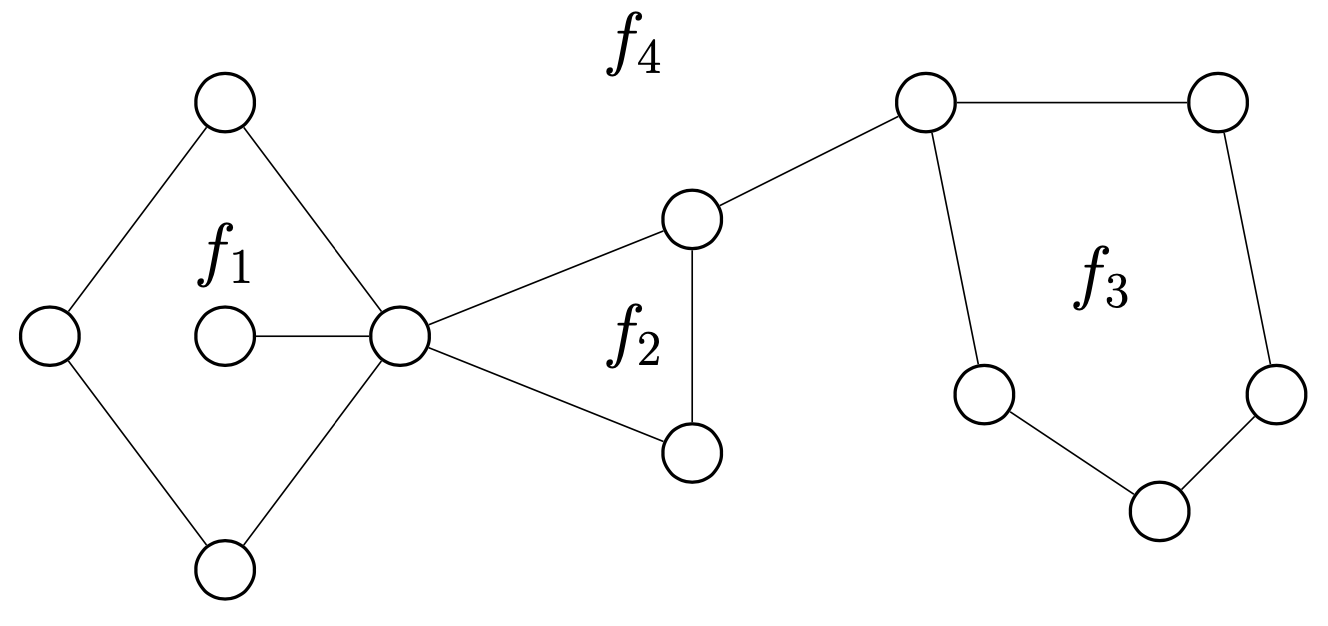
\includegraphics[scale=0.4]{Figures/Faces.png}
\end{center}
Tip: Think of a face as being the result of the bucket function in MS Paint. 
\subsubsection{Faceshaking Lemma}
$$2e = \sum_{f \in F(G)} deg(f)$$
In planar embeddings, $e$ is a bridge iff two sides of $e$ are in the same face. 
\subsubsection{Jordan Curve Theorem}
Every planar embedding separates the plane into two parts, one on the outside (exterior) and one on the inside (interior). 

\subsection{Duals}
A planar embedding has a corresponding dual $G^*$ which is constructed as follows: $G^*$ has one vertex for each face of $G$. Two vertices of $G^*$ are joined by an edge whenever the corresponding faces of $G$ have an edge in common (one side for each face), and the edge in $G^*$ is drawn to cross this common boundary edge in $G$. 
\begin{center}
    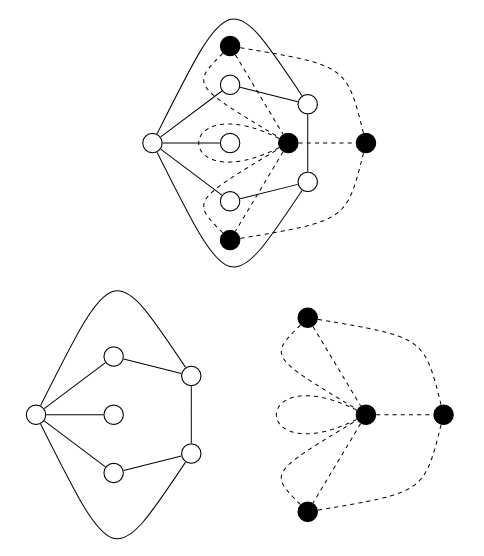
\includegraphics[scale=0.70]{Figures/Dual.png}
\end{center}
If $G$ is connected, then $G = (G^*)^*$ 

\subsection{Euler's Formula}
\subsubsection{Definition}
For all connected planar embeddings the following will always hold, 
$$n-m+s = 2$$

\subsubsection{Euler's Inequality (Formula for Non-connected Graphs)}
$$n -m + s = 1 + c \geq 2$$ 
$Proof \: Sketch.$ Connecting $c$ components adds $c-1$ edges while not increasing the number of faces. Adding bridges does not change the planarity since $e$ is surrounded by the outer face on both sides. So with our new $m$, we substitute $n- (m+c-1) +s = 2$ which yields the inequality as needed. \hfill \qedsymbol \nl
If $G$ is planar s.t. $\forall$ faces have degree at least $d^* \geq 3$, then 
\begin{align*}m \leq \frac{d^*}{d^*-2}(n-2) \tag*{$(Lem \: 7.5.2)$}\end{align*}
If $G$ is planar and contains a cycle, then the boundary of each face contains a cycle $(Lem)$.
\begin{eg}{Show that $\forall$ planar embeddings has a vertex of degree $\leq 5$ or a face of degree $\leq 3$.}
\vspace{-20pt}
\begin{proof}
 Assume that all faces have degree $\geq 3$. Then by Lemma 7.5.2 we have that
$$m \leq \frac{d^*}{d^*-2}(n-2) \implies m \leq \frac{3}{1}(n-2) = 3(n-2)$$
The average degree of a vertex is defined as
$$\frac{\sum_{v \in V(G)} deg(v)}{n} = \frac{2m}{n} \leq \frac{2(3(n-2))}{n} =  6 \cdot \frac{n-2}{n} < 6$$
So the average degree is less than 6, which implies there is a vertex with degree at most 5.
\end{proof}
\end{eg}
\subsection{Certifying Nonplanar Graphs}
\subsubsection{Using Inequalities}
In a non-bipartite planar $G$ with $p \geq 3$ vertices and $q$ edges, we have $$q \leq 3p - 6$$
In a bipartite planar $G$ with $p \geq 3$ vertices and $q$ edges, we have $$q \leq 2p - 4$$
All planar graphs have a vertex of degree at most 5 ($Cor$). \nl 
So to certify non-planarity, we can show that these inequalities do not hold.  
\begin{eg}{Show that $K_5$ is a non-planar graph.}
\vspace{-10pt}
$Corollary.$
By the Lemma, 
$$\binom{5}{2} \leq 3(5) - 1 \implies 10 \leq 9$$ 
which clearly does not hold. $\therefore$ $K_5$ is not planar. \hfill \qedsymbol
\end{eg}
The same proof works for showing that $K_{3,3}$ is not planar as well. 
\subsubsection{Kuratowski's Theorem}
An edge subdivision of $G$ is obtained after each edge is independently replaced by a path of length 1 or more. \nl 
Using Kuratowski's Theorem, we can show that a graph is non-planar by showing that $G$ has a subgraph that is an edge subdivision of $K_5$ or $K_{3,3}$.\nl 
Tip: Identifying an odd cycle eliminates the possibility of $K_{3,3}$.

\subsection{Colouring and Planar Graphs}
A $k$-colouring of $G$ is an assignment of $k$ colours to all vertices of $G$ where adjacent vertices cannot be assigned the same colour. \nl
A graph with a $k$-colouring graph is $k$-colourable. Also, a $k$-colourable graph is $(k+1)$-colourable, $(k+2)$-colourable, and so on.
\subsubsection{Bipartite Graphs}
A graph is 2-colourable iff it's bipartite $(Thm \: 7.7.2)$. \nl 
$Proof \: Sketch.$ Given bipartition $(A,B)$, both directions involves setting all vertices of $A$ to be the first colour and $B$ the second colour. \hfill \qedsymbol
\subsubsection{6-Colour Theorem}
All planar graphs are 6-colourable ($Thm$). \nl
The proof is dependent on the fact that there exists a vertex with degree at most 5. 
\begin{proof} Assume that $G$ is a planar graph. The proof is by induction on $n$ vertices where $P(n)$ is the statement that $G$ is 6-colourable. \nl 
\textbf{Base Case:} All planar graphs on one vertex are 6-colourable, so the result is true for $n = 1$. \nl 
\textbf{Inductive Hypothesis:} Assume that $\forall$ planar graphs are 6-colourable for $k \leq n$ vertices, where $k \geq 1$. \nl
\textbf{Inductive Step:} Consider $G$ such that there are $n = k + 1$ vertices. By a Lemma, we know that all planar embeddings have at least one vertex $v$ with $deg(v) \leq 5$. Suppose we remove vertex $v$, and all edges incident to $v$ from $G$. We denote this resulting graph as $G'$. Then $G'$ has $k$ vertices, and is a planar graph since all subgraphs of a planar graph are also planar. We apply the inductive hypothesis to $G'$, so $G'$ is 6-colourable. Now find a 6-colouring of $G'$. There are at most 5 vertices in $G'$ that are adjacent to $v$ in $G$, so these vertices are assigned at most 5 different colours in the 6-colouring of $G$. Thus there is at least one of the 6 colours remaining. Assign one of these remaining colours to $v$, so that $v$ has a different colour from all of its adjacent vertices in $G$. Thus we have a 6-colouring of $G$, and the result is true for $n = k + 1$. We have now proved that the result is true by POMI.
\end{proof}
\subsubsection{5-Colour Theorem}
Edge contraction for edge $e = {x,y}$ is an operation that allows the length of $e$ to decrease to 0 s.t. vertices $x$ and $y$ are identified as a new a vertex $z = xy$ and produces a new graph $H = G / e$. 
\begin{center}
    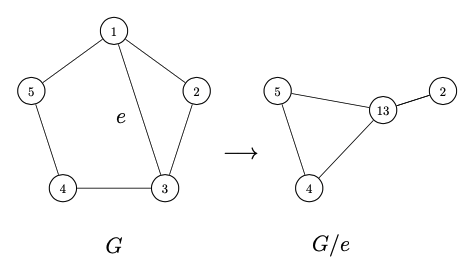
\includegraphics[scale=0.50]{Figures/Contraction.png}
\end{center}
All planar graphs are 5-colourable ($Thm$). 
\begin{proof}
Assume that $G$ is a planar graph. The proof is by induction on $n$ vertices. \nl 
\textbf{Base Case:} All planar graphs on one vertex are 5-colourable, so the result is true for $n = 1$. \nl
\textbf{Inductive Hypothesis:} Assume that all planar graphs on $n \leq k$ vertices are 5-colourable s.t. $k \geq 1$. \nl 
\textbf{Inductive Step:} We consider two cases of $G$ for $n = k + 1$ vertices: \nl 
{\underline{Case I:}} $G$ has a vertex of degree at most 4 \nl 
Use same argument as the 6-colour theorem proof. \nl 
{\underline{Case II:}} $G$ has no vertex of degree at most 4 ($G$ is minimum degree 5) \nl
This implies that $G$ has a vertex $v$ of degree 5 (since $\forall$ planar embeddings have a vertex of degree at most 5 and we assumed that there does not exist a vertex of at most degree 4). Furthermore, all 5 adjacent vertices of $v$ cannot be mutually adjacent as otherwise we would have a $K_5$ subgraph which contradicts our assumption that $G$ is planar. So there are at least two vertices $x, y \in N_G(v)$ that are not adjacent.
Contract edge $\{x, v\}$ to obtain $H = G / e$ and label the new vertex as $v$, then contract $\{y, v\}$ to obtain $K = H / e$ and label the new vertex as $v$. As $G$ is planar, we know that $H$ and $K$ is as well; moreover, $K$ has $k + 1 - 2 = k-1$ vertices and thus $K$ is 5-colourable by the inductive hypothesis. Use the 5-colouring of $K$ to colour all the vertices of $G$ except for $x, y,$ and $v$. We know that $x$ and $y$ are not adjacent in $G$, so they can be assigned the same colour. Colour both vertices $x$ and $y$ in $G$ with the colour assigned to vertex $v$ in $K$. Hence, at most four distinct colours appear on the five neighbours of $v$. Colour $v$ with one of the absent colours. Then we have a valid 5-colouring of $G$. \nl
In both cases, G has a 5-colouring. Therefore, by mathematical induction it follows that every planar graph has a 5-colouring.
\end{proof}

\subsubsection{4-Colour Theorem}
All planar graphs are 4-colourable ($Thm$).

\newpage
\section{Matchings}
\subsection{Matching}
A matching $M$ of $G$ is a set of edges s.t. each edge in $M$ share no common vertices. \nl 
Vertices in $M$ are saturated by the matching. \nl 
A maximum matching is the largest matching possible in $G$; a perfect matching is a type of maximum matching s.t. all vertices of $G$ are saturated and $\therefore$ has size $\frac{n}{2}$. \nl 
An alternating path is a path s.t. consecutive edges alternate in $M$ and not being in $M$; an augmenting path is a type of alternating path that starts and ends in distinct unsaturated vertices (of odd length).
\subsection{Covers}
A cover $C$ of $G$ is a set of vertices that have at least one endpoint of all edges in $G$. \nl
In any graph, $|M| \leq |C|$ ($Lem$). \nl 
If $|M| = |C|$, then $M$ is a maximum matching and $C$ is a minimum cover ($Lem$).

\begin{eg}{Say $M$ is a maximum matching and $C$ is a minimum cover of $G$.
Show $|C| \leq 2|M |$.}
\vspace{-20pt}
\begin{proof}
Let $G = (V, E)$ be a graph such that $M$ is the corresponding maximum matching and $C$ is the corresponding minimum cover. Given $M$, there are $2|M|$ saturated vertices by a definition of a matching. Notice that the 2$|M|$ saturated vertices of $M$ forms a vertex cover $C^*$ for $G$. Otherwise, if $C^*$ is not a cover then there would exist an edge $e$ that can then be added to $M$ since $e$ would not be incident to any saturated vertices in $C^*$ which would contradict our assumption that $M$ is a maximum matching. Moreover, $C^*$ is not necessarily a minimum cover so 
$$|C| \leq |C^*| = 2|M|$$
which proves the statement as desired.
\end{proof}
\end{eg}

\subsection{K\"onig's Theorem}

In all bipartite graphs, the maximum size of a matching is the minimum size of a cover.

\subsubsection{Bipartite Matching Algorithm: XY-Construction}
We say that $G$ has the cover $C = Y \cup (A \setminus X)$. \nl 
The $XY$-construction tries to keep finding augmenting paths and flipping them until there are no more. \nl 
The current iteration stops and the next iteration begins when we find an unsaturated vertex in $Y$. \nl 
Halting Condition of $XY$-Construction: 
\begin{enumerate}[(1)]
    \item $X_0$ is empty. 
    \item We cannot go from $X \rightarrow Y$.  
\end{enumerate} 
\begin{eg}{Apply the matching algorithm with $M$ as an initial matching ($A = \{1,2,3,4\}$).}
\vspace{-20pt}
\begin{center}
    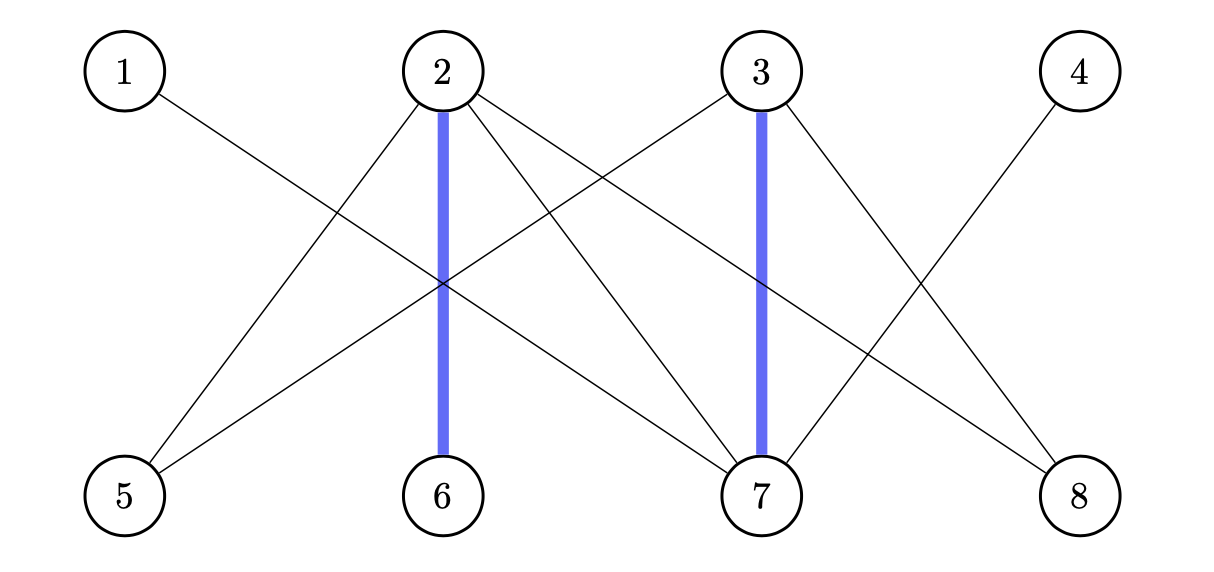
\includegraphics[scale=0.40]{Figures/XYConstruct.png}
\end{center}
\vspace{-15pt}
\underline{Iteration 1:} \nl
$X_0 = \{1, 4\}$ \nl 
$Y = \{7\}$ ; pr(7) = 1,4 \nl 
$X = \{3\}$ ; pr(3) = 7 \nl 
$Y = \{5, 8 \}$ ; pr(5) = pr(8) = 3 \nl
5 is unsaturated. STOP. \nl Flip augmenting path: $$5371$$
\underline{Iteration 2:} \nl
$X_0 = \{4\}$ \nl
$Y = \{7\}$ ; pr(7) = 4 \nl
$X = \{1\}$ ; pr(1) = 7 \nl
STUCK.\nl 
Now $Y \cup (A \setminus X) = \{2, 3, 7\}$ and $M = \{\{17\}, \{38\}, \{26\}\}$ so therefore
$$|M| = 3 = |Y \cup (A \setminus X)|$$
\end{eg}
Tip:
\begin{itemize}
    \lstspacing
    \item $X \rightarrow Y$ 
    \item $Y \leadsto X$
\end{itemize}  

\subsection{Application of Hall's Theorem}

\subsubsection{Hall's Theorem}
Hall's Condition is satisfied if $\forall(D \subseteq A)$ 
that $|N(D)| \geq |D|$. If Hall's Condition holds, then by Hall's Theorem there exists a matching that saturates $A$. \nl
If $G$ is bipartite where Hall's Condition is satisfied and $|A| = |B|$ then $G$ has a perfect matching. \nl 
Every $k$-regular graph has a perfect matching. 
\begin{eg}{Consider a standard deck of cards in a $4 \times 13$ array. Show that it is possible to pick one card from each column such that we get all 13 values.}
\vspace{-20pt}
\begin{proof}
Consider a graph $G$ with bipartition ($A, B$). Let $A = \{A, 2, 3, \dots, J, Q, K\}$ and $B = \{1, 2, \dots, 11, 12, 13\}$. That is, $A$ contains all 13 card values and $B$ contains all of the columns where a vertex $x \in A$, $y \in B$ are adjacent if the card value $x$ is in column $y$. To prove the statement it is sufficient to show that $A$ has a perfect matching. Take a subset $D \subseteq B$ of $k$ columns. Notice that there are $4k$ cards in these columns, and each value has at most 4 cards which implies that at least $k$ values exist. So Hall's condition holds and there is therefore a perfect matching.
\end{proof}
\end{eg}

\subsection{Edge Colouring}
An edge $k$-colouring of a graph $G$ is an assignment of one of a set of $k$ colours to each edge of $G$ so that two edges incident with the same vertex are assigned different colours. \nl 
A bipartite graph with at most degree $\delta$ has an edge $\delta$-colouring ($Thm. \:$ 8.7.1). 
\end{document}
